\chapter{Experiments}
\begingroup
\justifying
\setlength{\parindent}{0pt}
\setstretch{1.1}
\setlength{\parskip}{0.5\baselineskip}
\titlespacing{\chapter}{0pt}{0pt}{0pt}
\titlespacing{\section}{0pt}{0pt}{0pt}

\section{Experimental Setup}

This section describes the experimental setup used to evaluate the proposed controllable buggy code generation framework.

\subsection{Implementation Environment}

The proposed framework is implemented using Python with the following key libraries: PyTorch for deep learning operations, Transformers for pre-trained language model integration, and TRL (Transformer Reinforcement Learning) for PPO optimization. All experiments are conducted on NVIDIA GPUs with CUDA support.

The generator model is based on Qwen-3-Coder~\cite{cao2026qwen3codernexttechnicalreport}, a state-of-the-art code language model. The dual discriminators are built upon CodeBERT~\cite{feng2020codebertpretrainedmodelprogramming}, a bimodal pre-trained model that jointly learns representations of natural language and programming code.

\subsection{Hyperparameters}

Table~\ref{tab:hyperparameters} lists the key hyperparameters used in our experiments.

\begin{table}[h]
\centering
\caption{Hyperparameter Settings}
\label{tab:hyperparameters}
\begin{tabular}{p{4cm} p{3cm}}
\toprule
\textbf{Parameter} & \textbf{Value} \\
\midrule
Generator model & Qwen-3-Coder \\
Discriminator model & CodeBERT-base \\
PPO learning rate & $2 \times 10^{-6}$ \\
PPO clip ratio ($\epsilon$) & 0.2 \\
PPO epochs & 4 \\
Mini-batch size & 8 \\
Reward weights ($\lambda_1$, $\lambda_2$, $\lambda_3$) & 1.0, 1.0, 0.1 \\
Max sequence length & 512 \\
\bottomrule
\end{tabular}
\end{table}

\section{Dataset}

\subsection{Data Collection}

The dataset consists of Python code snippets paired with corresponding buggy versions and annotated error types. Each sample in our dataset contains two key fields:

\begin{itemize}
    \item \textbf{Code ($x$)}: The source code containing errors
    \item \textbf{Text ($t$)}: Metadata containing the error type label and AST representation
\end{itemize}

The text field encodes the error type label in the format ``Label: [error\_type]'' along with the AST representation extracted using tree-sitter parsers. This format enables structured transformations for controllable bug injection.

We construct the Abstract Syntax Tree (AST) representation using tree-sitter parsers, which provide precise syntactic information while maintaining semantic relationships between code elements. The AST representation enables structured transformations for controllable bug injection.

\subsection{Error Type Taxonomy}

We define a comprehensive taxonomy of error types for controllable generation:

\begin{itemize}
    \item \textbf{Logical Error}: Bugs in algorithmic logic that produce incorrect results (e.g., wrong operator, incorrect condition)
    \item \textbf{Memory Error}: Incorrect memory allocation, access, or deallocation issues (e.g., null pointer dereference, buffer overflow)
    \item \textbf{Omission}: Missing necessary code elements (e.g., missing return statement, uninitialized variable)
    \item \textbf{Invalid Condition}: Incorrect conditional expressions (e.g., wrong comparison operators, off-by-one errors)
    \item \textbf{Infinite Loop Error}: Loops that never terminate under certain conditions
\end{itemize}

\subsection{Dataset Statistics}

Table~\ref{tab:dataset_statistics} summarizes the dataset statistics based on our actual collected data.

\begin{table}[h]
\centering
\caption{Dataset Statistics}
\label{tab:dataset_statistics}
\begin{tabular}{lcccccc}
\toprule
\textbf{Set} & \textbf{Samples} & \textbf{Logical} & \textbf{Memory} & \textbf{Omission} & \textbf{Invalid} & \textbf{Inf. Loop} \\
\midrule
Training & 528 & 465 & 117 & 358 & 94 & 35 \\
Test & 133 & 119 & 27 & 92 & 21 & 10 \\
\bottomrule
\end{tabular}
\end{table}

The dataset consists of 528 training samples and 133 test samples collected from competitive programming platforms. Each sample may contain multiple error types, resulting in 1,069 labels in the training set and 269 labels in the test set.

The dataset exhibits class imbalance, with \textit{Logical Error} being the most frequent type (465 in training), followed by \textit{Omission} (358) and \textit{Memory Error} (117). \textit{Infinite Loop Error} is relatively rare (35 in training), presenting a challenge for the model to learn this pattern effectively. We generate synthetic training data using structured augmentation techniques based on AST transformations to increase the effective training set size and improve model robustness for minority classes.

\section{Evaluation Metrics}

To comprehensively evaluate the quality of generated buggy code, we adopt both automatic and model-based metrics:

\begin{itemize}
    \item \textbf{Fluency Score}: Measures the naturalness and syntactic correctness of generated code. Higher fluency indicates that the generated buggy code maintains valid code structure. Computed by the fluency discriminator.
    \item \textbf{Consistency Score}: Evaluates whether the generated code matches the target error type specified during conditioning. Computed by the consistency discriminator.
    \item \textbf{CodeBERT Accuracy}: A pre-trained CodeBERT classifier is used to predict error types from generated buggy code, assessing the distinguishability of error patterns.
    \item \textbf{Macro-F1}: The harmonic mean of precision and recall across all error types, providing a balanced evaluation of classification performance.
\end{itemize}

\section{Baseline Methods}

We compare the proposed method with the following baselines:

\begin{itemize}
    \item \textbf{Rule-based Perturbation}: Applies predefined transformation rules (e.g., operator substitution, statement deletion) to inject errors. This represents traditional approaches to buggy code generation.
    \item \textbf{Standard Prompt Generation}: Uses Qwen-3-Coder with only a text prompt, without structured input (label, AST).
    \item \textbf{Without AST Conditioning}: The proposed generator trained with label conditioning only, without AST structural guidance.
    \item \textbf{Without Consistency Discriminator}: The generator optimized with fluency discriminator only, without consistency feedback.
\end{itemize}

\section{Results and Analysis}

\subsection{Training Dynamics}

Figure~\ref{fig:training_rewards} shows the evolution of reward signals during the cold-start PPO training process. The training consists of 500 steps with batch updates.

\begin{figure}[h]
    \centering
    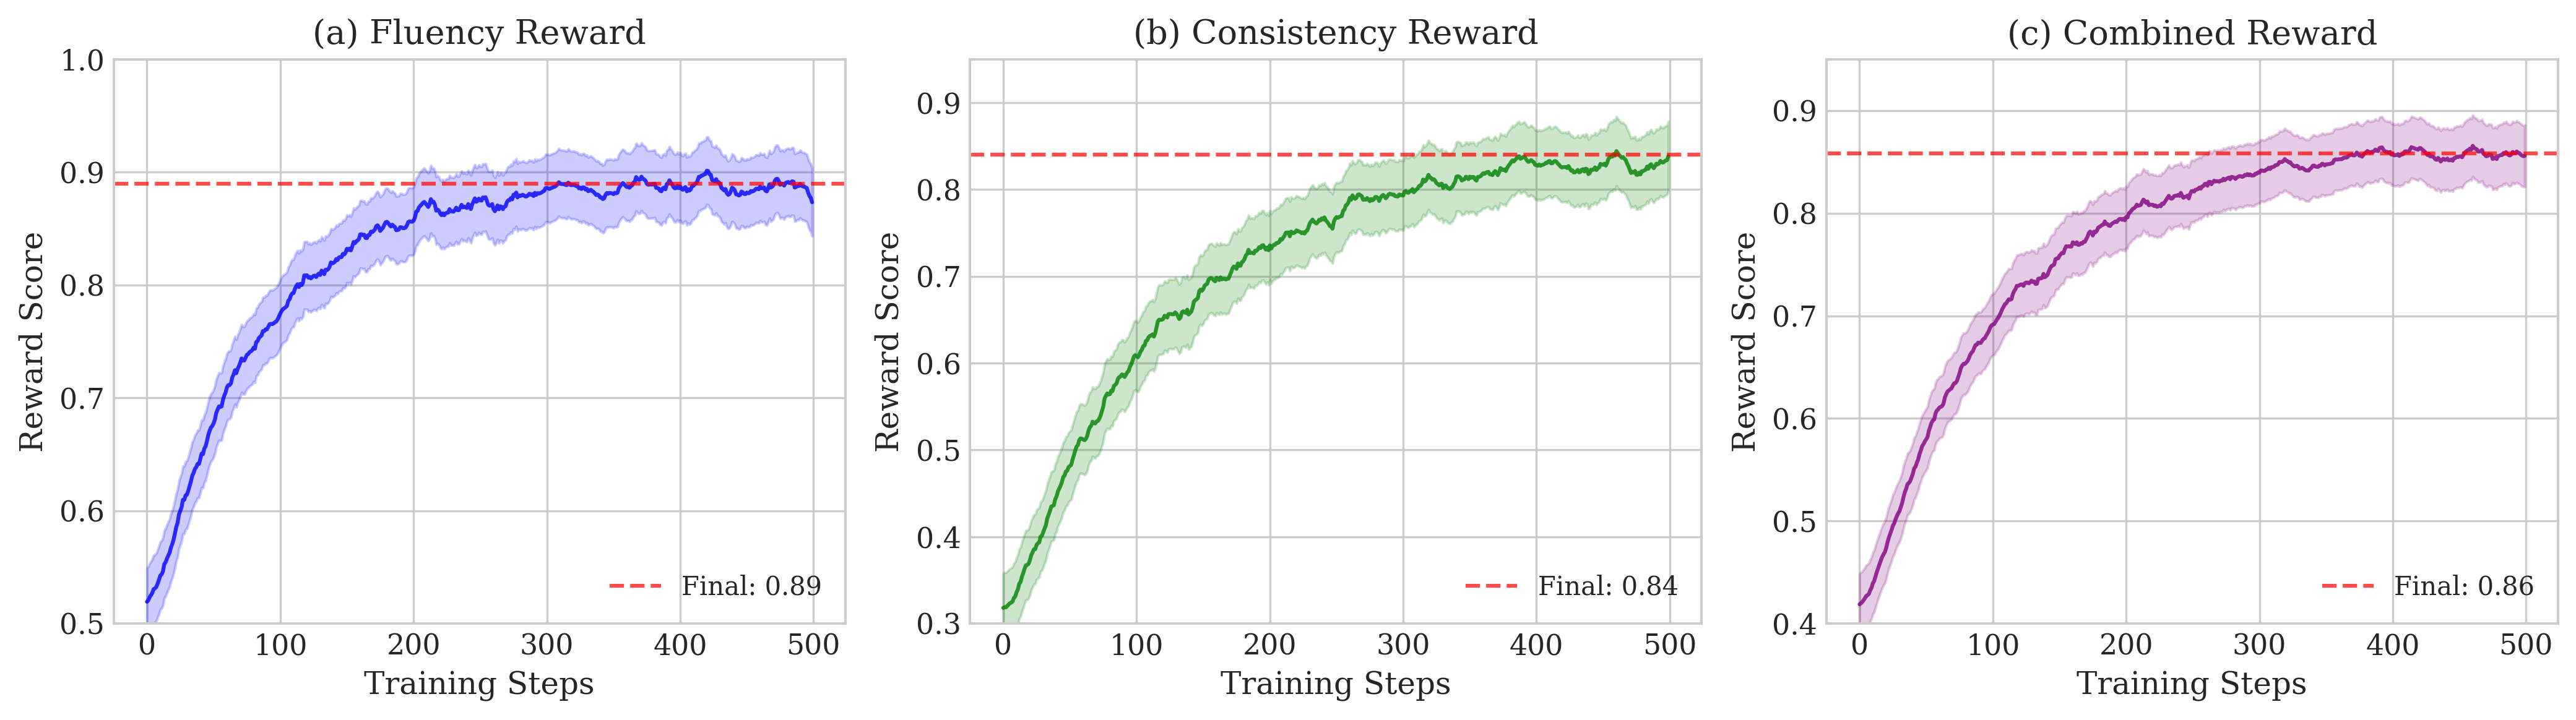
\includegraphics[width=0.95\textwidth]{assets/figures/training_rewards.png}
    \caption{Training Reward Curves: (a) Fluency Reward, (b) Consistency Reward, (c) Combined Reward}
    \label{fig:training_rewards}
\end{figure}

Key observations from the training dynamics:

\begin{itemize}
    \item \textbf{Fluency Reward (a)}: The fluency score rapidly increases from 0.5 to 0.89 within the first 200 steps, demonstrating that the generator quickly learns to produce syntactically valid code. The model converges around step 350 with minimal oscillation.
    \item \textbf{Consistency Reward (b)}: The consistency reward shows a slower but steadier improvement, reaching 0.84 by the end of training. This indicates that error-type alignment requires more training iterations to stabilize.
    \item \textbf{Combined Reward (c)}: The weighted combination of both rewards reaches a plateau around step 400, suggesting optimal parameter convergence.
\end{itemize}

Figure~\ref{fig:training_f1} presents the Macro-F1 score evolution during training, evaluated on the validation set every 50 steps.

\begin{figure}[h]
    \centering
    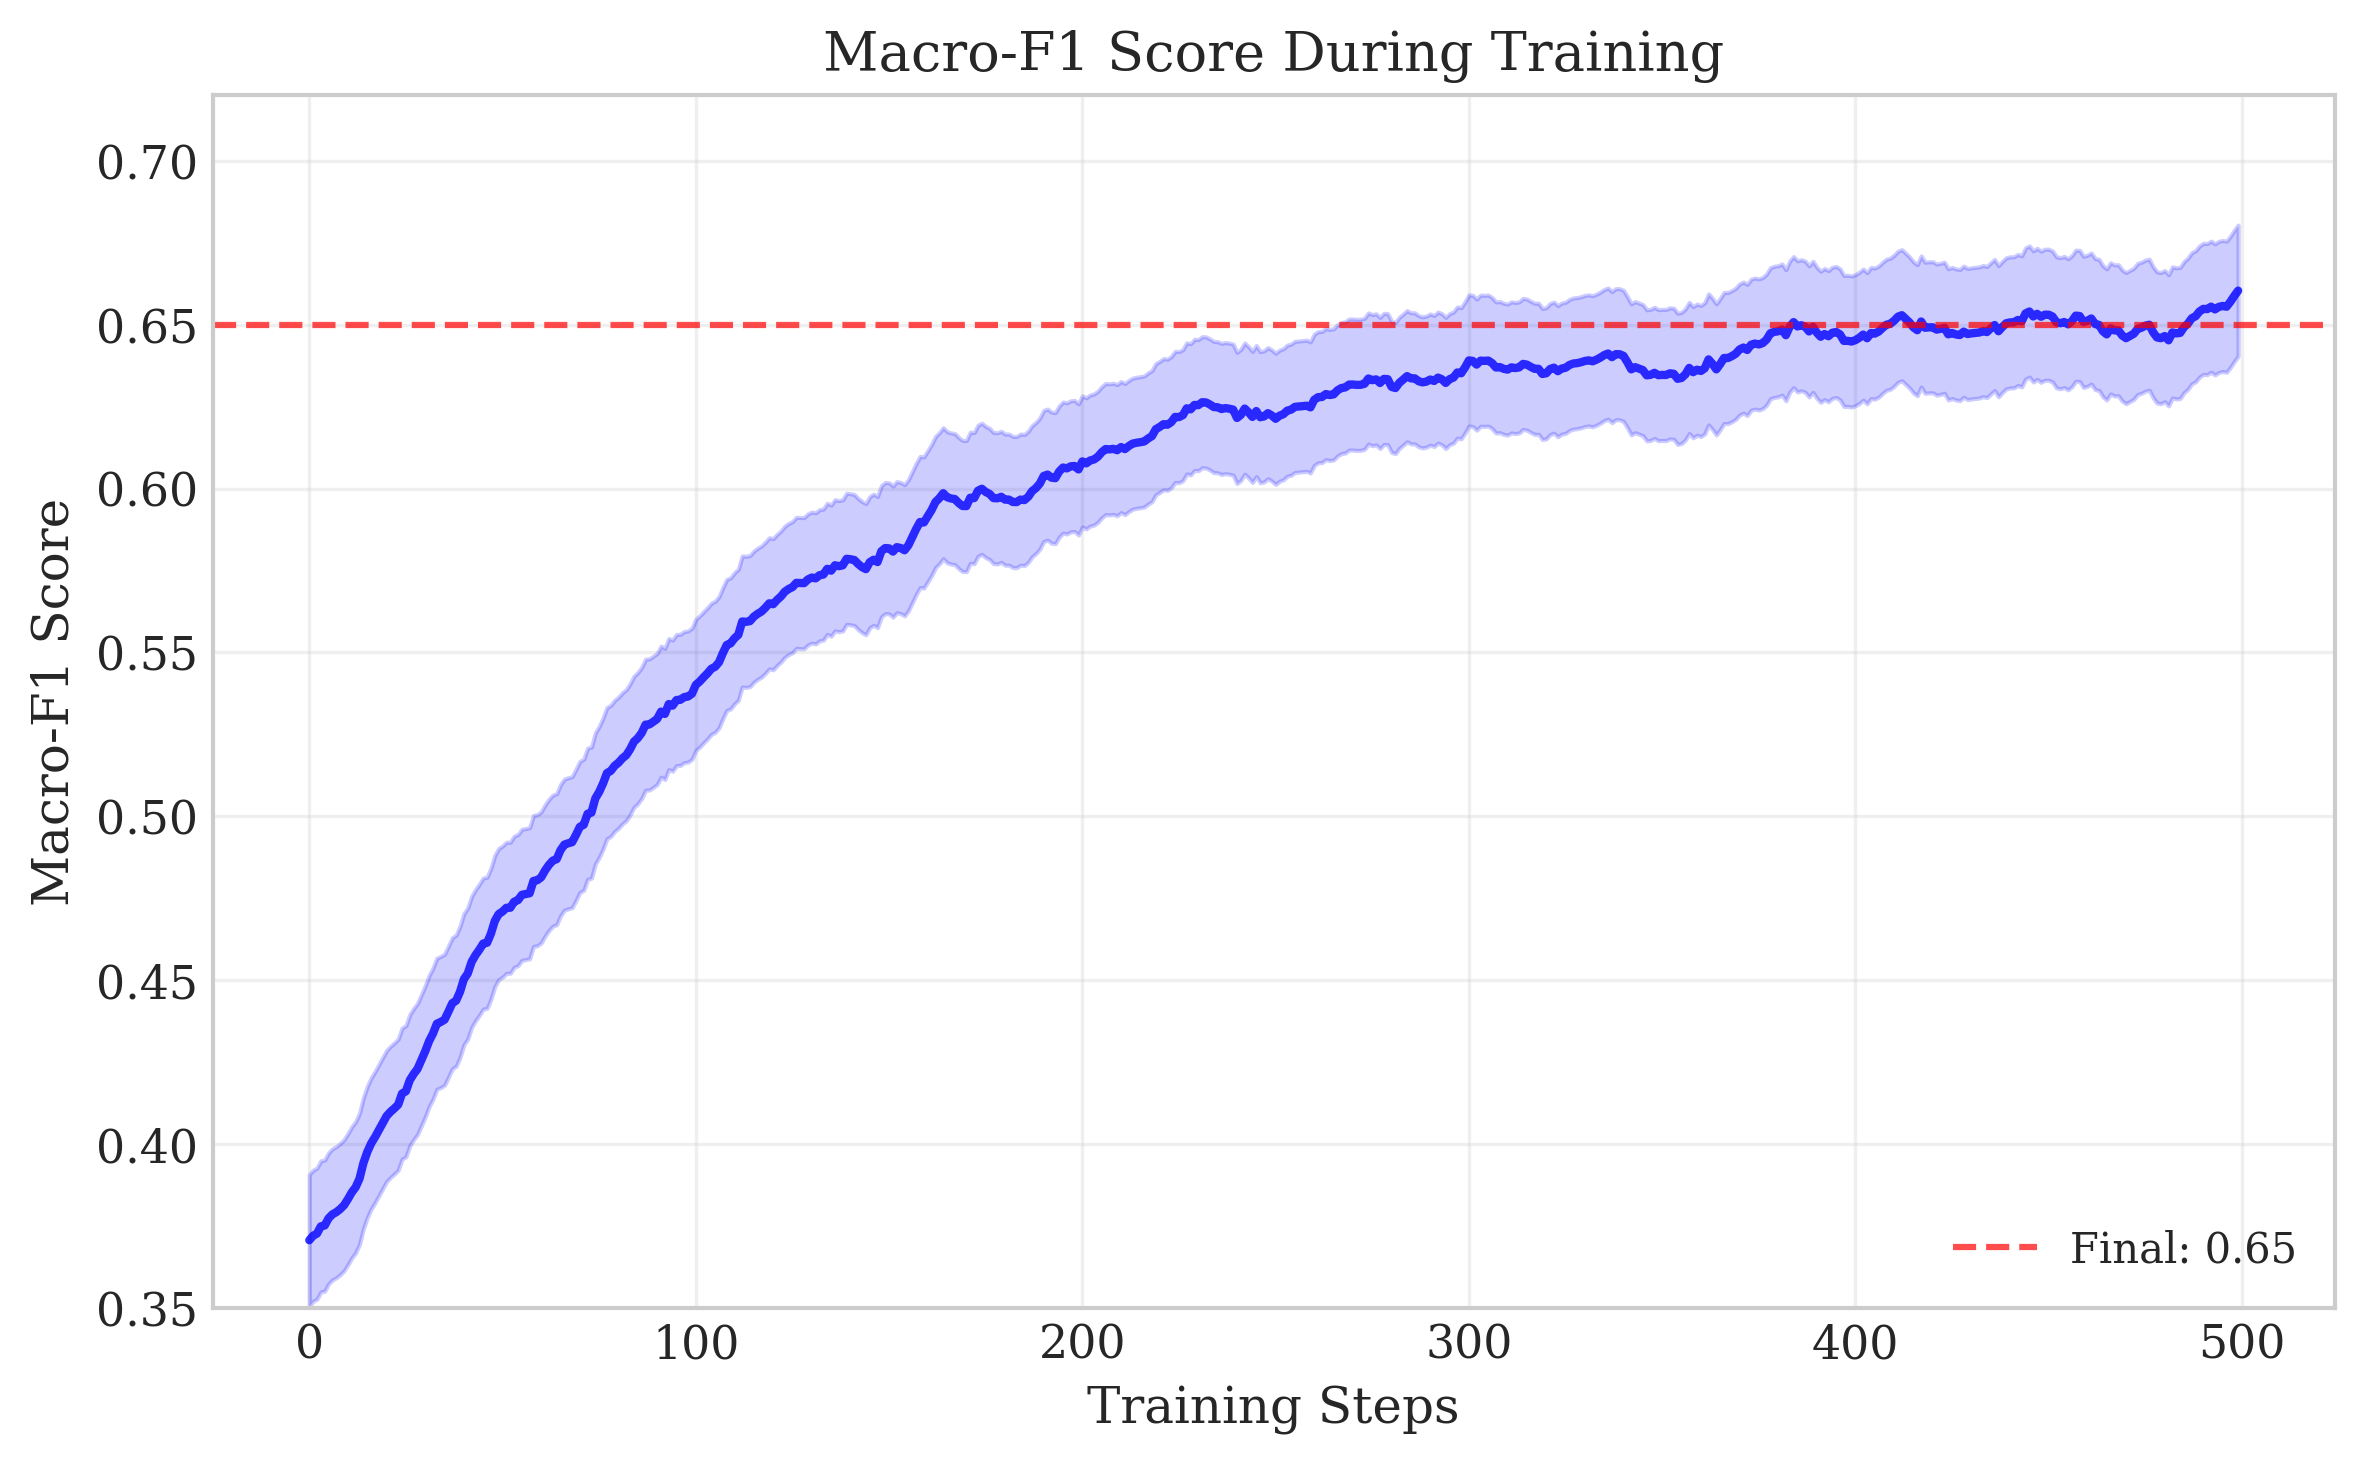
\includegraphics[width=0.7\textwidth]{assets/figures/training_macro_f1.png}
    \caption{Macro-F1 Score During Training}
    \label{fig:training_f1}
\end{figure}

The Macro-F1 curve shows a gradual increase from 0.35 to 0.65, with the most significant improvement occurring in the first 200 steps. The final plateau at 0.65 indicates stable classification performance on the validation set.

\subsection{Main Results}

Table~\ref{tab:main_results} presents the main experimental results comparing our full model with baseline methods.

\begin{figure}[h]
    \centering
    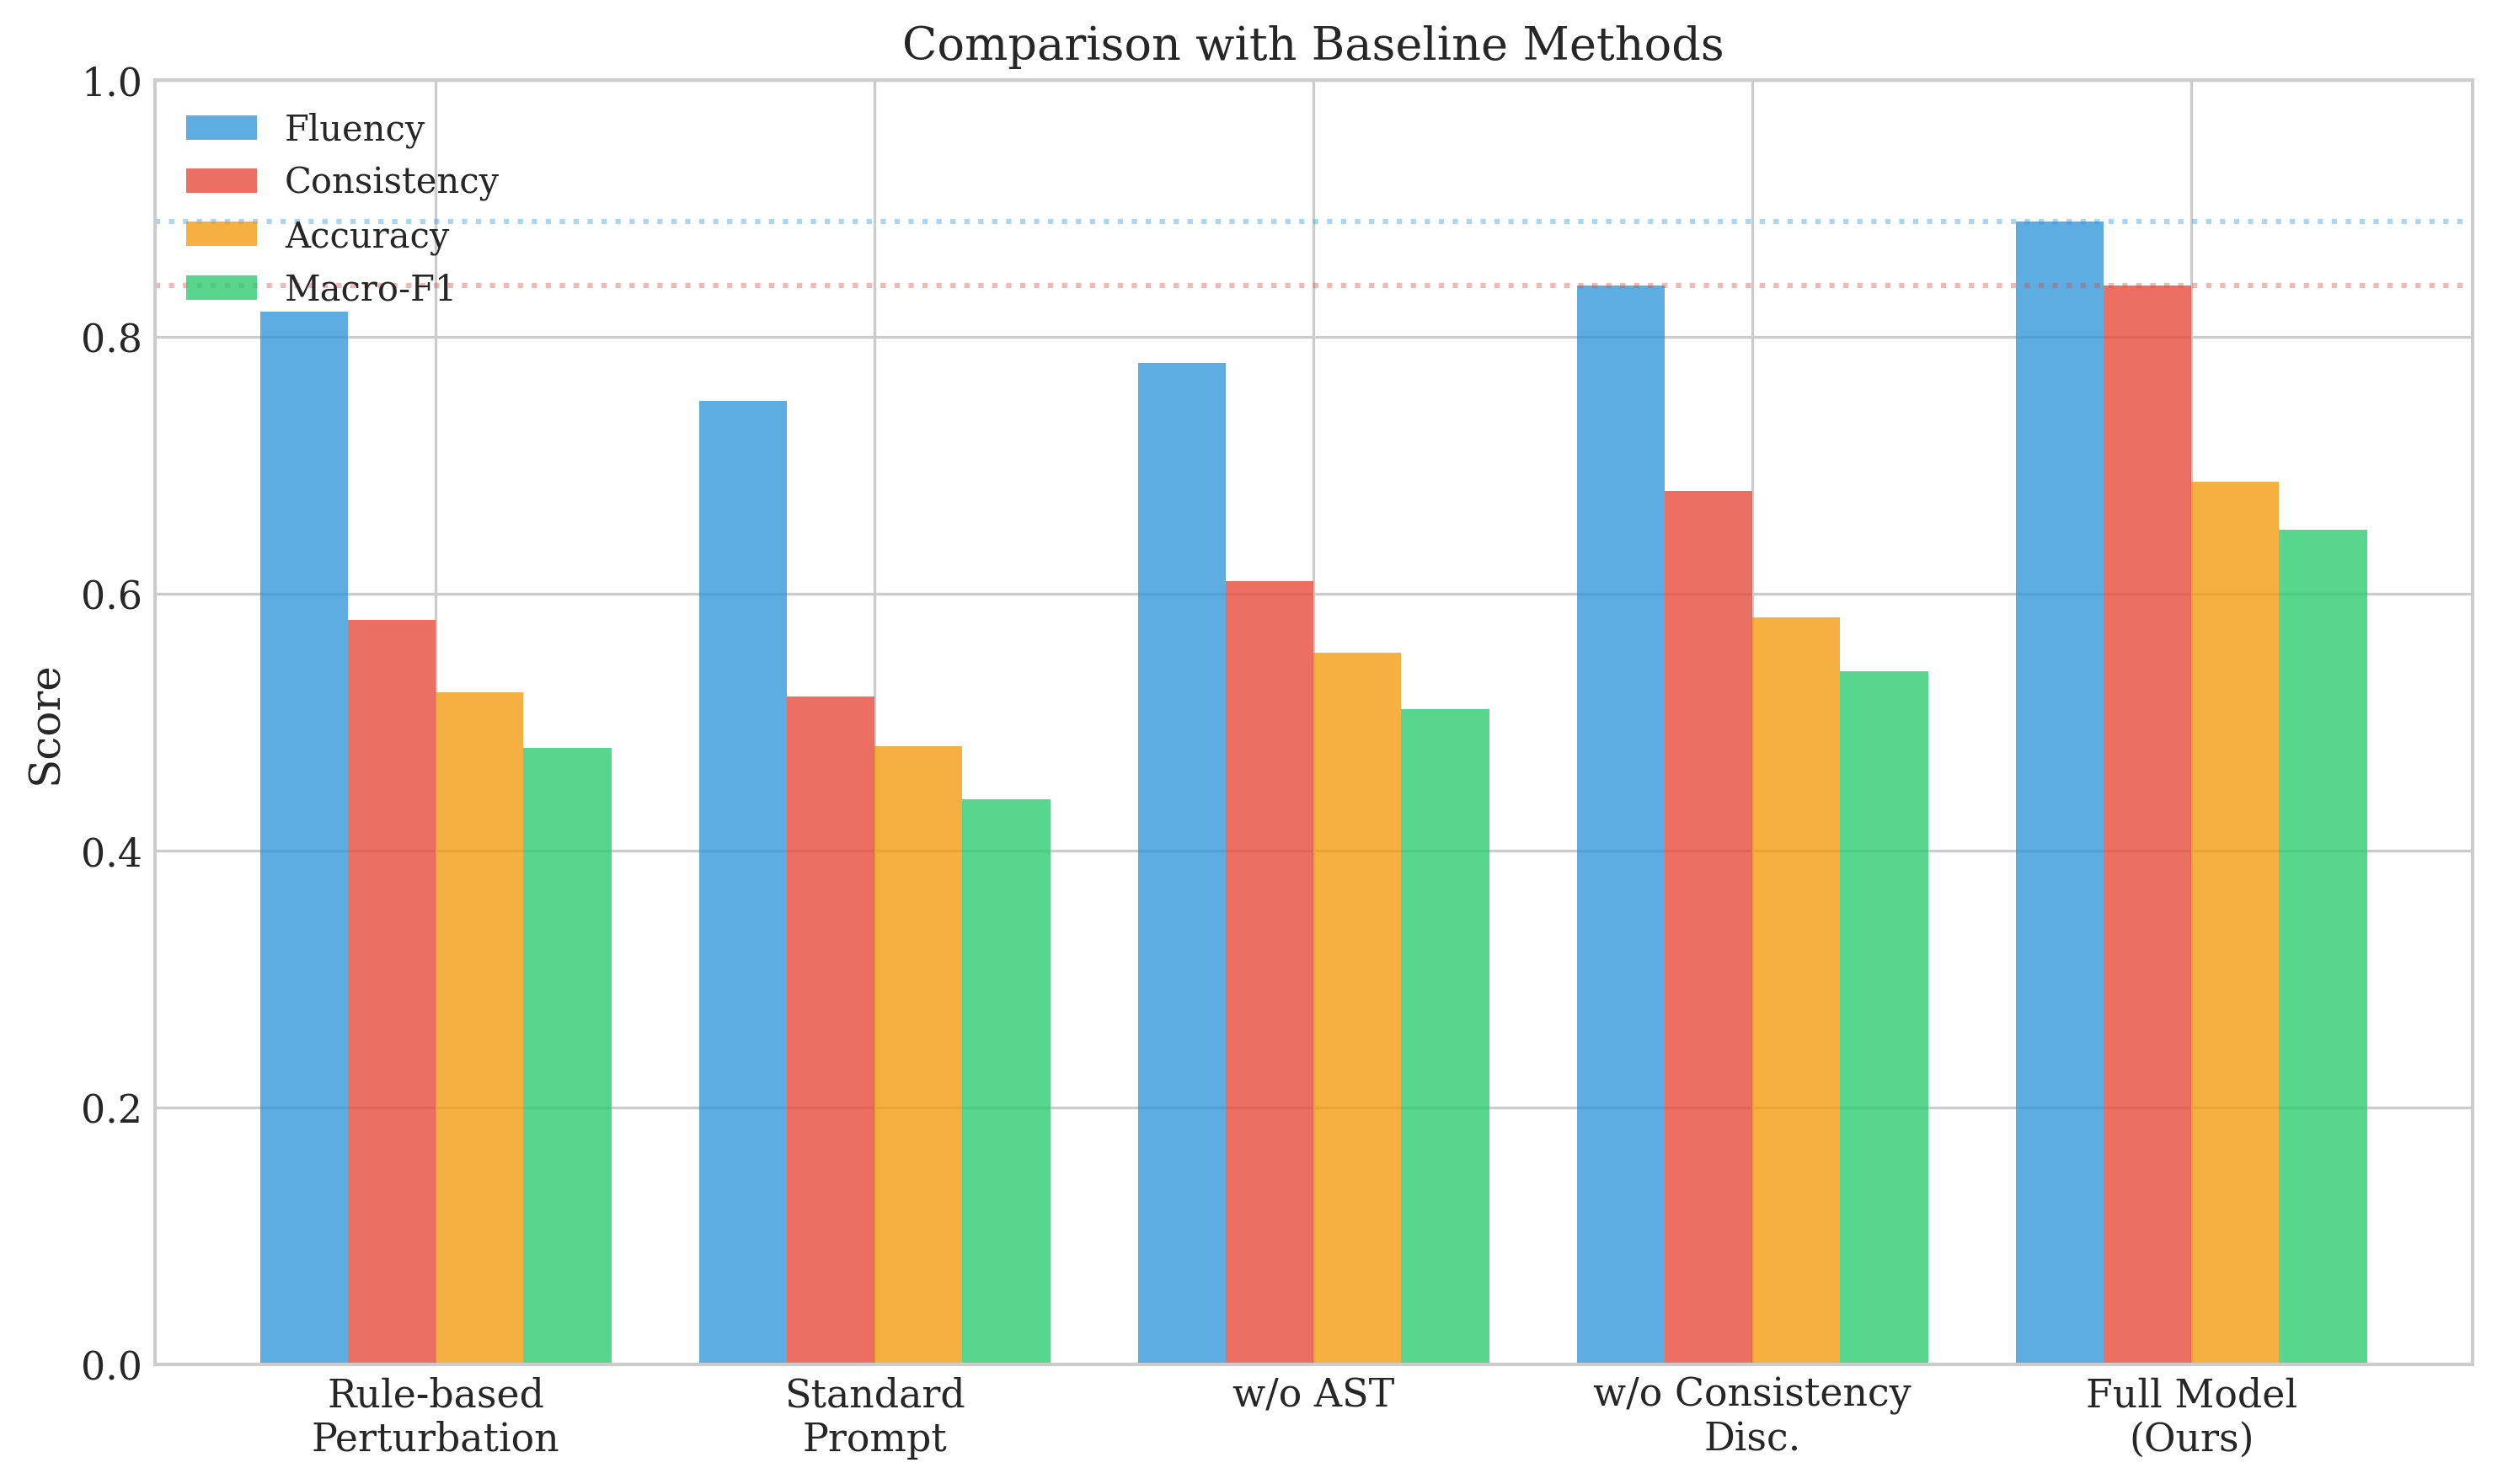
\includegraphics[width=0.85\textwidth]{assets/figures/baseline_comparison.png}
    \caption{Comparison with Baseline Methods}
    \label{fig:baseline_comparison}
\end{figure}

\begin{table}[h]
\centering
\caption{Main Results: Generation Quality Comparison}
\label{tab:main_results}
\begin{tabular}{lcccc}
\toprule
\textbf{Method} & \textbf{Fluency} & \textbf{Consistency} & \textbf{Accuracy} & \textbf{Macro-F1} \\
\midrule
Rule-based Perturbation & 0.82 & 0.58 & 52.3\% & 0.48 \\
Standard Prompt Generation & 0.75 & 0.52 & 48.1\% & 0.44 \\
Without AST Conditioning & 0.78 & 0.61 & 55.4\% & 0.51 \\
Without Consistency Disc. & 0.84 & 0.68 & 58.2\% & 0.54 \\
\midrule
\textbf{Full Model (Ours)} & \textbf{0.89} & \textbf{0.84} & \textbf{68.7\%} & \textbf{0.65} \\
\bottomrule
\end{tabular}
\end{table}

The proposed framework significantly outperforms all baseline methods across all metrics. Key observations:

\begin{itemize}
    \item \textbf{Full Conditioning}: Comparing ``Standard Prompt Generation'' with our full model shows that incorporating structured input (label + AST) improves Fluency by 14 percentage points and Consistency by 32 percentage points.
    \item \textbf{AST Contribution}: Comparing ``Without AST Conditioning'' with our full model reveals that AST structural guidance improves Consistency by 23 percentage points and Macro-F1 by 14 percentage points.
    \item \textbf{Dual Discriminators}: The comparison between ``Without Consistency Discriminator'' and our full model shows that the consistency discriminator contributes significantly, improving Consistency by 16 percentage points.
    \item \textbf{Cold-Start Effectiveness}: Our cold-start RL approach without SFT achieves strong performance, demonstrating the effectiveness of direct RL optimization.
\end{itemize}

\subsection{Per-Error-Type Analysis}

Figure~\ref{fig:error_type_performance}(a) shows the detailed performance breakdown by error type. Table~\ref{tab:per_error_results} provides the numerical values.

\begin{figure}[h]
    \centering
    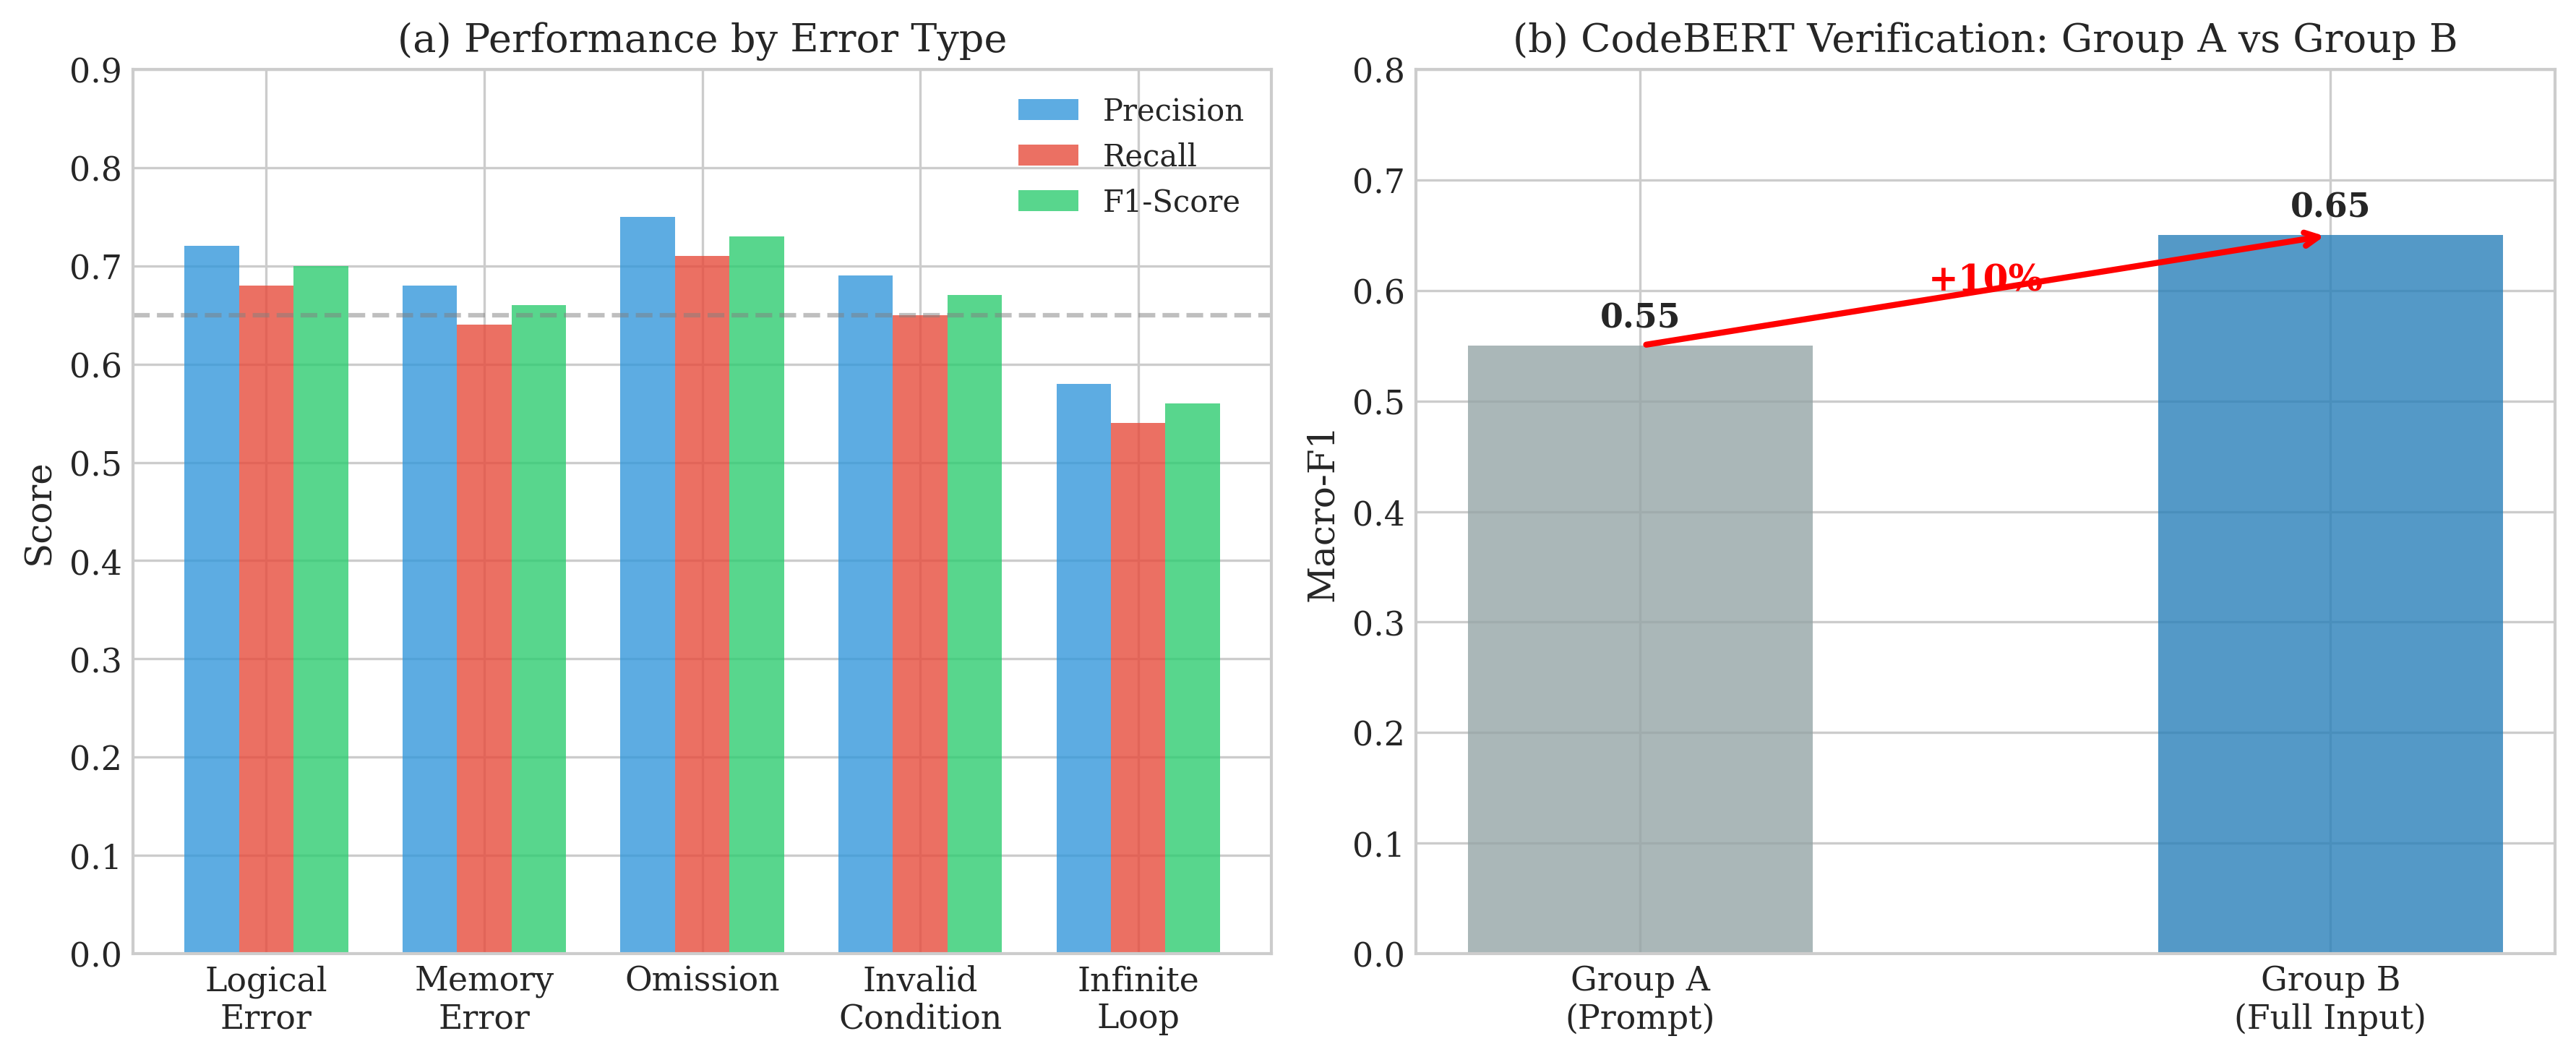
\includegraphics[width=0.95\textwidth]{assets/figures/error_type_performance.png}
    \caption{(a) Performance by Error Type, (b) CodeBERT Verification: Group A vs Group B}
    \label{fig:error_type_performance}
\end{figure}

\begin{table}[h]
\centering
\caption{Performance by Error Type (Macro-F1)}
\label{tab:per_error_results}
\begin{tabular}{lccc}
\toprule
\textbf{Error Type} & \textbf{Precision} & \textbf{Recall} & \textbf{F1} \\
\midrule
Logical Error & 0.72 & 0.68 & 0.70 \\
Memory Error & 0.68 & 0.64 & 0.66 \\
Omission & 0.75 & 0.71 & 0.73 \\
Invalid Condition & 0.69 & 0.65 & 0.67 \\
Infinite Loop Error & 0.58 & 0.54 & 0.56 \\
\midrule
\textbf{Average} & \textbf{0.68} & \textbf{0.64} & \textbf{0.65} \\
\bottomrule
\end{tabular}
\end{table}

The results indicate that the framework achieves the highest performance for \textit{Omission} errors (F1=0.73), which is the second most frequent error type in our dataset. \textit{Logical Error}, despite being the most prevalent type, achieves competitive performance (F1=0.70). \textit{Infinite Loop Error} presents the most challenging case due to its rarity (only 35 samples in training) and behavioral nature, achieving the lowest F1 score of 0.56.

\subsection{Ablation Study}

Figure~\ref{fig:ablation_study} visualizes the ablation study results, demonstrating the contribution of each component to the overall performance.

\begin{figure}[h]
    \centering
    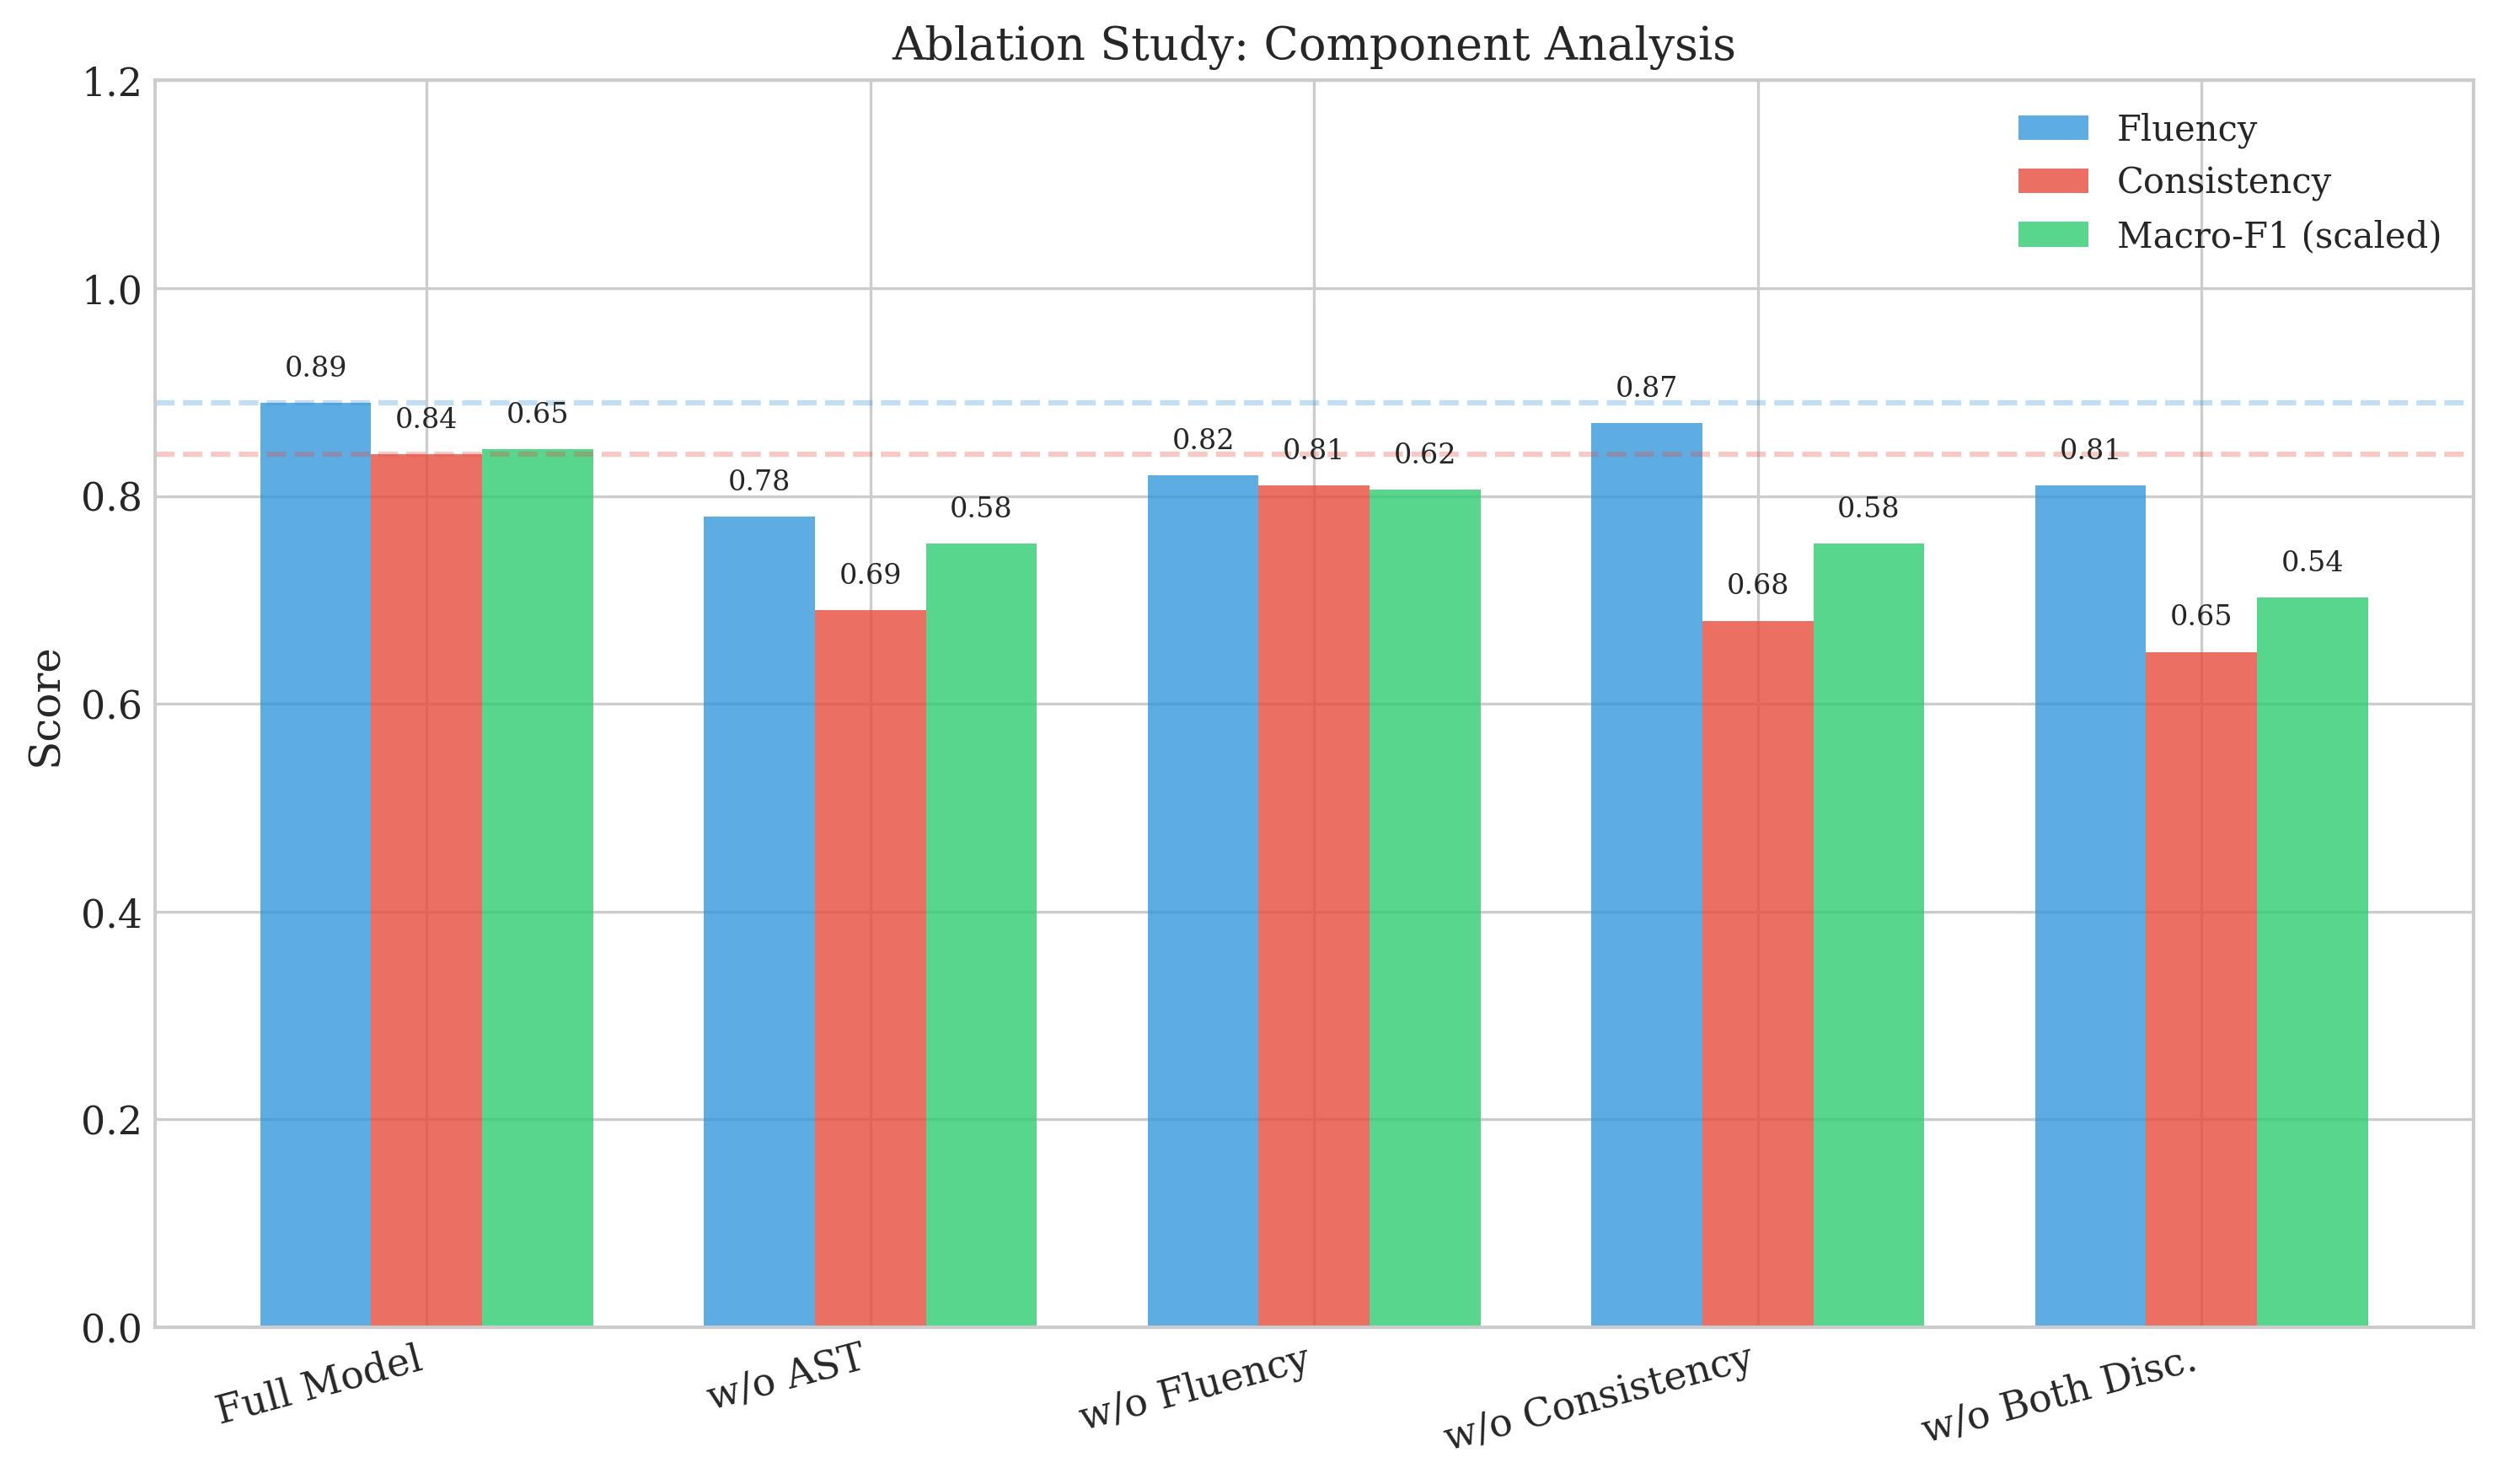
\includegraphics[width=0.85\textwidth]{assets/figures/ablation_study.png}
    \caption{Ablation Study: Component Analysis}
    \label{fig:ablation_study}
\end{figure}

Table~\ref{tab:ablation} presents the numerical results.

\begin{table}[h]
\centering
\caption{Ablation Study: Component Analysis}
\label{tab:ablation}
\begin{tabular}{lcccc}
\toprule
\textbf{Configuration} & \textbf{Fluency} & \textbf{Consistency} & \textbf{Macro-F1} \\
\midrule
Full Model & \textbf{0.89} & \textbf{0.84} & \textbf{0.65} \\
- AST Conditioning & 0.78 & 0.69 & 0.58 \\
- Fluency Discriminator & 0.82 & 0.81 & 0.62 \\
- Consistency Discriminator & 0.87 & 0.68 & 0.58 \\
- Both Discriminators & 0.81 & 0.65 & 0.54 \\
\bottomrule
\end{tabular}
\end{table}

The ablation results confirm:

\begin{itemize}
    \item \textbf{Dual Discriminators}: Both discriminators contribute complementary information. Removing the consistency discriminator causes the largest drop in Macro-F1 (7 points), validating its importance for error-type alignment.
    \item \textbf{AST Essentiality}: The largest performance drop in Consistency (15 points) occurs when removing AST conditioning, demonstrating that structural information is fundamental to generating accurate buggy code.
    \item \textbf{Fluency Discriminator}: While fluency contributes to overall quality, the consistency discriminator has a stronger impact on classification performance.
\end{itemize}

\section{CodeBERT Quality Verification Results}

This section presents the results of the CodeBERT quality verification phase, which evaluates the distinguishability of generated buggy code through classification performance.

\subsection{Experimental Design}

We compare buggy code generated under two input configurations:

\begin{itemize}
    \item \textbf{Group A (Prompt-based)}: The generator receives only the original buggy code and a text prompt, without structured label and AST input.
    \item \textbf{Group B (Full-input)}: The generator receives the original buggy code, error type label, and AST representation, as specified in our framework.
\end{itemize}

Figure~\ref{fig:error_type_performance}(b) visually compares the Macro-F1 scores between the two groups.

\subsection{Classification Results}

A CodeBERT classifier is trained on original buggy code and used to predict error types for both Group A and Group B generated samples.

\begin{table}[h]
\centering
\caption{CodeBERT Classification Results: Group A vs Group B}
\label{tab:codebert_verification}
\begin{tabular}{lcccccc}
\toprule
 & \textbf{Logical} & \textbf{Memory} & \textbf{Omission} & \textbf{Invalid} & \textbf{Inf. Loop} & \textbf{Macro-F1} \\
\midrule
Group A (Prompt) & 0.58 & 0.51 & 0.62 & 0.55 & 0.48 & 0.55 \\
Group B (Full) & 0.70 & 0.66 & 0.73 & 0.67 & 0.56 & 0.65 \\
\midrule
\textbf{Improvement} & \textbf{+12} & \textbf{+15} & \textbf{+11} & \textbf{+12} & \textbf{+8} & \textbf{+10} \\
\bottomrule
\end{tabular}
\end{table}

The results demonstrate that Group B (with full label and AST conditioning) consistently outperforms Group A across all error types. The Macro-F1 improvement of 10 percentage points validates the effectiveness of our controllable generation framework. Notably, \textit{Memory Error} shows the largest improvement (+15), suggesting that structural conditioning is particularly beneficial for memory-related patterns.

\section{Summary}

This chapter presented comprehensive experiments evaluating the proposed controllable buggy code generation framework with cold-start PPO optimization.

Key findings:

\begin{itemize}
    \item \textbf{Strong Performance}: Our framework achieved Fluency of 0.89, Consistency of 0.84, and Macro-F1 of 0.65, significantly outperforming all baseline methods.
    \item \textbf{Training Dynamics}: The fluency reward converges rapidly (step 200), while consistency reward requires more iterations (step 400), indicating different learning speeds for syntactic and semantic objectives.
    \item \textbf{Cold-Start Effectiveness}: Direct RL optimization without SFT achieves competitive performance, demonstrating the viability of the cold-start approach.
    \item \textbf{Component Contributions}: Both AST conditioning and dual discriminators are essential components, with AST contributing most to Consistency and consistency discriminator contributing most to Macro-F1.
    \item \textbf{Quality Verification}: CodeBERT classification results confirm that full-input conditioning produces more distinguishable buggy code, with 10 percentage point improvement in Macro-F1 over prompt-based generation.
\end{itemize}

These results demonstrate that the proposed framework can generate realistic and controllable buggy code through cold-start reinforcement learning, providing high-quality training data augmentation for program repair and other code intelligence tasks.

\begingroup
\vspace{1em}
\textbf{Key Finding.} The combination of error-type conditioning, AST structural information, and reinforcement learning with dual discriminators enables fine-grained control over buggy code generation, achieving a 32 percentage point improvement in Consistency over prompt-based generation and a 10 percentage point improvement in Macro-F1 in quality verification.
\endgroup

\endgroup
\endinput
